\chapter{Starting to Decode}

In our last lab, you finished the first stage of our pipeline, Fetch, by adding a buffer.  Now we are going to move on to the first two components of the decode stage.

\section{Sign Extender}
Consider the code in Listing~\ref{code:se}.  It really has only one new line, which shows two uses of curly braces: concatenation and replication.  Concatenation is done by \verb1{a,b}1, which would concatenate the bits of a with the bits of b to form a longer sequence.  Replication is done by \verb1n{a}1, which copies a n times.  If you look at our code it takes a number that is half a word long, and makes it a full word by copying the most significant bit.  The replication is made generic by using the constant WORD, and calculating the bit locations.  Unfortunately, the bit location (index) and number of times to copy it (n) have yet to be entered.

\Verilog{Verilog code to build a sign extender.}{code:se}{../code/sign_extender.v}


\section{Control Unit}
The control unit is the brains of our operation.  It will have to take the first six bits of every instruction (the opcode), and set the control bits.

First lets discuss what signals we are setting.  Almost all the boolean signals are described in Figure~\ref{fig:signals}.  The tricky one in the table is PCSrc, which can't be calculated yet, since we need to know whether the condition of the branch was met.  All we know at the moment is that it is a branch, so that is the signal the control will send. Later after the condition has been checked in the execute stage, we can combine the branch signal with the result of the condition to generate PCSrc.  ALUop is not described, though the value of both its bits is, since it is not a boolean signal.  ALUop is a signal that tells the alu control unit, which we will build in the execute stage, what to do or to check the function field.

\begin{figure}
\caption{Control signal meanings and values.}\label{fig:signals}
\begin{center}
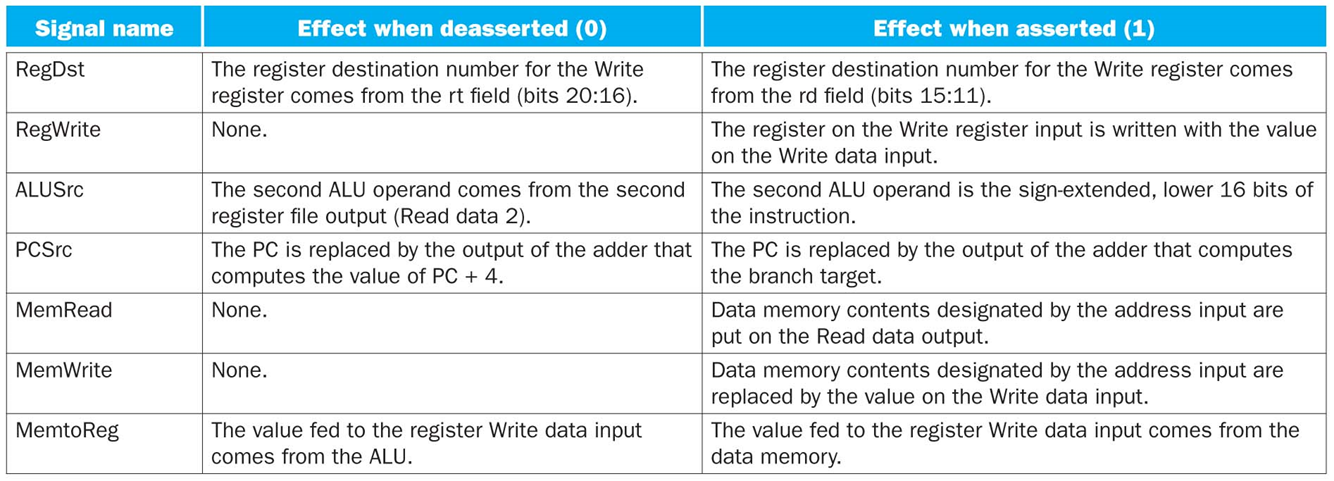
\includegraphics[width=\textwidth]{../images/signal_meaning.png}\\
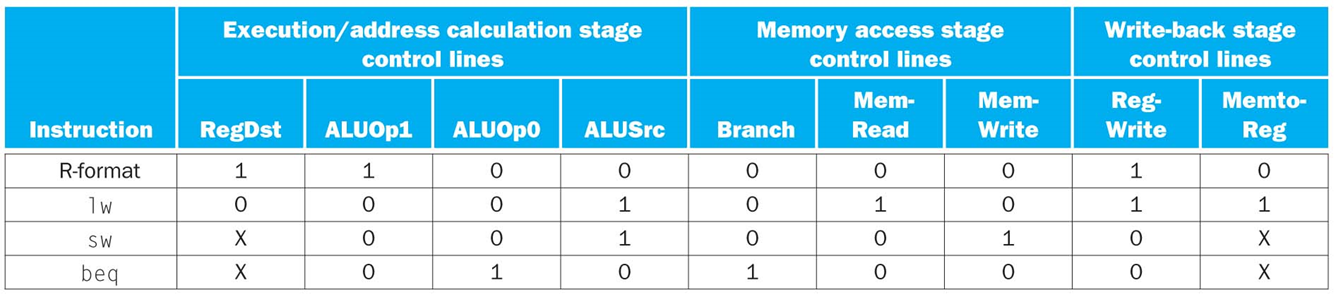
\includegraphics[width=\textwidth]{../images/control_lines.png}
\end{center}
\end{figure}

Consider the code in Listing~\ref{code:control}.  We introduce the switch statement, since it is the fastest way to check an integer indexed group of things, both in hardware and software.  The other well known alternative is a group of nested if-then-else statements.  In hardware\footnote{This is similar for software, where if you code it well you can get log base 2 evaluations on average.} this makes a series of nested 2-input muxes, which means there will be log base 2 levels of muxes to go through.  In complexity lingo, this is $O(\log(n))$ in time (how long it takes), and $O(1)$ in space (how big each mux is).  A case statement is similar to a switch-case statement in C.  In hardware\footnote{In software, this makes a branch table which takes no conditions and only a single branch to resolve!} this makes a single large mux, which thus has only one level of evaluation.  In complexity lingo this is $O(1)$ in time, and $O(n)$ in space.  We care about time, so we will go with the case statement.  Our case statement is missing the signal values, which you can fill in from Figure~\ref{fig:signals}.  Note I have defined the ALUop values as constants to improve readability, so you should use them (see definitions.vh for the names).

\Verilog{Verilog code for the control unit.}{code:control}{../code/control.v}

\section{Your Assignment}

You are to:
\begin{enumerate}
\item Finish the sign extender and control unit.
\item Write a testbench for the sign extender and control unit, run them and generate the timing diagram.
\item  Write up a lab report in \LaTeX\ following the lab format in \verb1LabN.tex1 and generate a pdf file.
\item Upload the pdf and all the Verilog files to the course LMS.
\end{enumerate} 